% 2015 | UIBK
% vim:set spell tw=79:

\documentclass[beamer]{uibk}
\title{SLIP}
\subtitle{RFC 1055 \\ Serial Line Internet Protocol}
\author{A. Fedrigolli, R. Gritzer, M. Pfeifhofer }
\date{\today}

\hypersetup{colorlinks,
            citecolor=black,
            filecolor=black,
            linkcolor=black,
            urlcolor=black}
\graphicspath{{./media/}}

\newcommand\textbox[1]{%
  \parbox{.333\textwidth}{#1}%
}

\usepackage{color}
\usepackage{tabto}
\usepackage{listings}
\usepackage{lipsum}

\definecolor{listinggray}{gray}{0.9}
\definecolor{lbcolor}{rgb}{0.9,0.9,0.9}

\lstset{backgroundcolor=\color{lbcolor},
    tabsize=4,
    language=C,
    basicstyle=\scriptsize,
    upquote=true,
    aboveskip={1.5\baselineskip},
    columns=fixed,
    showstringspaces=false,
    extendedchars=false,
    breaklines=true,
    prebreak = \raisebox{0ex}[0ex][0ex]{\ensuremath{\hookleftarrow}},
    frame=single,
    numbers=left,
    showtabs=false,
    showspaces=false,
    showstringspaces=false,
    identifierstyle=\ttfamily,
    keywordstyle=\color[rgb]{0,0,1},
    commentstyle=\color[rgb]{0.026,0.112,0.095},
    stringstyle=\color[rgb]{0.627,0.126,0.941},
    numberstyle=\color[rgb]{0.205, 0.142, 0.73}}

\begin{document}

\maketitle

\begin{frame}{Problem}
  \begin{center}
  Wir schreiben das Jahr {\huge 1988!}
  \end{center}
\end{frame}

\begin{frame}{Problem?}
  \begin{center}
  
\includegraphics[width=\textwidth, height=\textheight ,keepaspectratio]{iheart.jpg}
  \end{center}
\end{frame}

\begin{frame}{Problem?}
  \begin{center}
  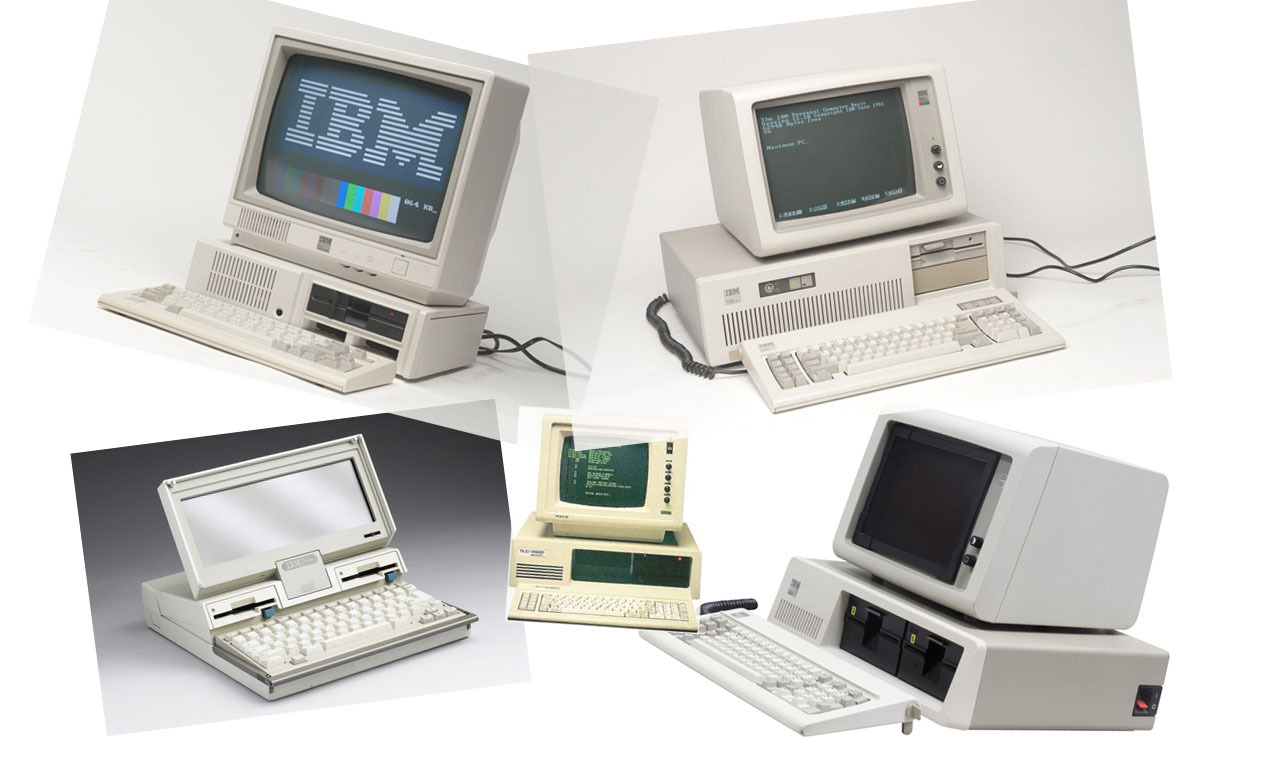
\includegraphics[width=\textwidth,height=\textheight,keepaspectratio]{1988computer.jpg}
  \end{center}
\end{frame}

\begin{frame}{Problem}
  \begin{center}
  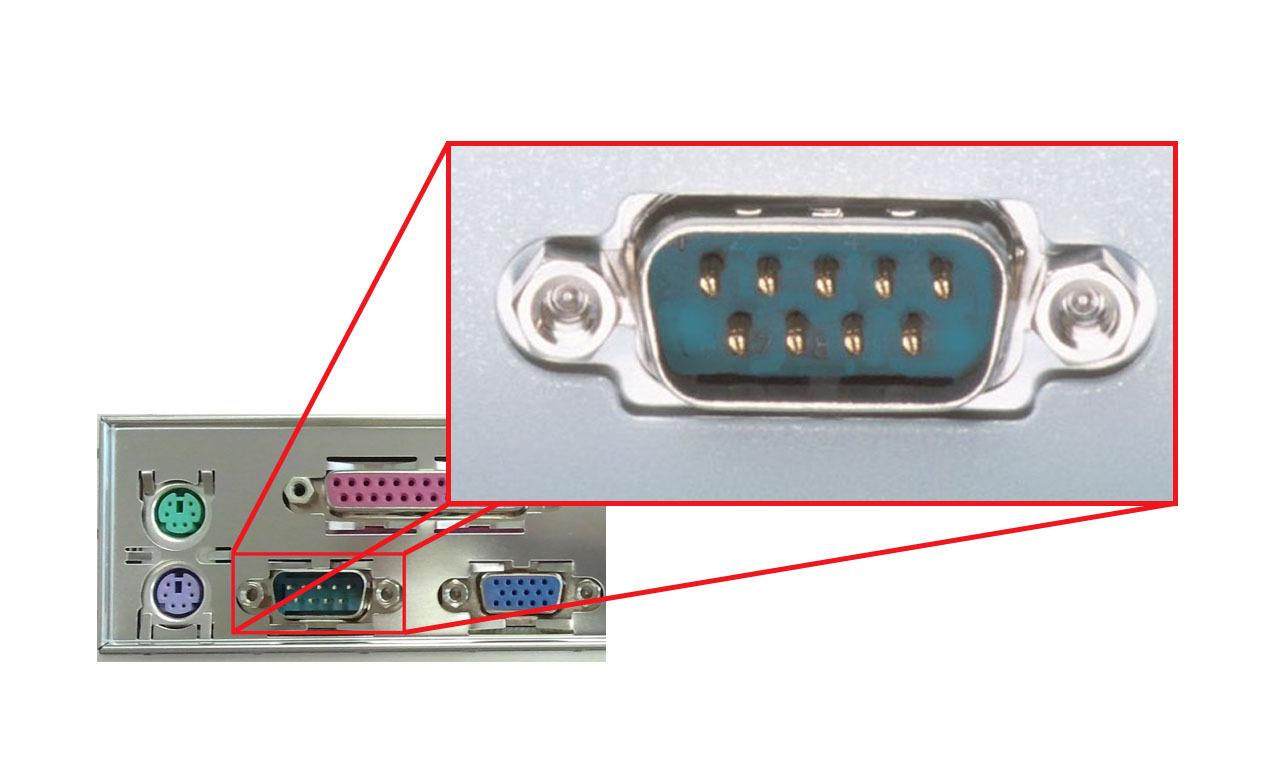
\includegraphics[width=\textwidth,height=\textheight,keepaspectratio]{serial.jpg}
  \end{center}
\end{frame}


\begin{frame}{Problem}
  \begin{center}
  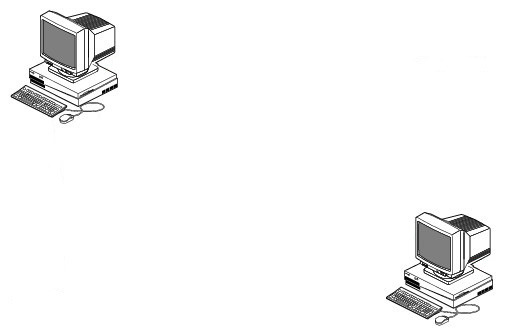
\includegraphics[width=\textwidth,height=\textheight,keepaspectratio]{ansatz_1.jpg}
  \end{center}
\end{frame}

\begin{frame}{Problem}
  \begin{center}
  
\includegraphics[width=\textwidth,height=\textheight,keepaspectratio]{ansatz_2.jpg}
  \end{center}
\end{frame}

\begin{frame}{Ansatz}
  \begin{center}
  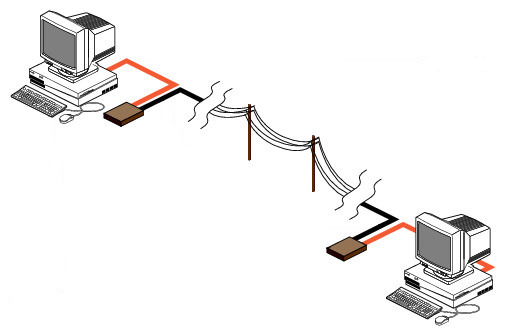
\includegraphics[width=\textwidth,height=\textheight,keepaspectratio]{ansatz_3.jpg}
  \end{center}
\end{frame}

\begin{frame}{Ansatz}
  \begin{center}
  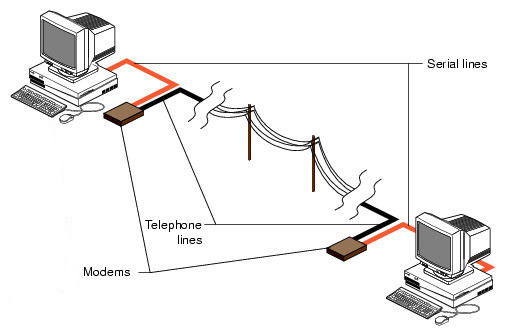
\includegraphics[width=\textwidth,height=\textheight,keepaspectratio]{ansatz_4.jpg}
  \end{center}
\end{frame}

\begin{frame}{Einordnung}
  \begin{center}
  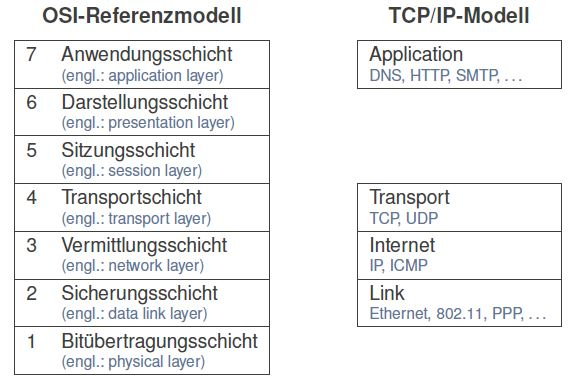
\includegraphics[width=\textwidth,height=\textheight,keepaspectratio]{layer.jpg}
  \end{center}
\end{frame}

\begin{frame}{Einordnung}
  \begin{center}
  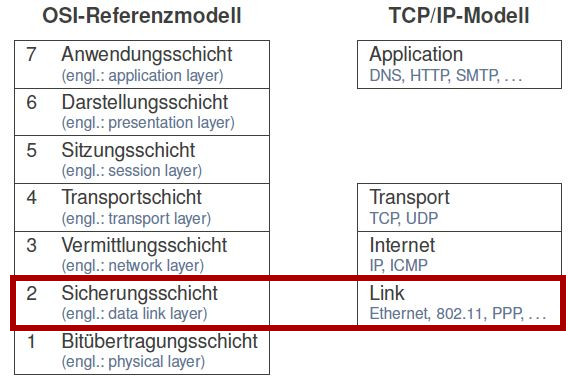
\includegraphics[width=\textwidth,height=\textheight,keepaspectratio]{layer2.jpg}
  \end{center}
\end{frame}

\begin{frame}{Aufbau}
  \newpage
  \begin{center}
  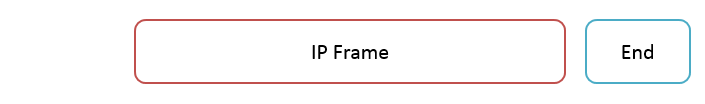
\includegraphics[width=\textwidth,height=\textheight,keepaspectratio]{ip1.png}
  \end{center}
\end{frame}

\begin{frame}{Aufbau}
  \newpage
  \begin{center}
  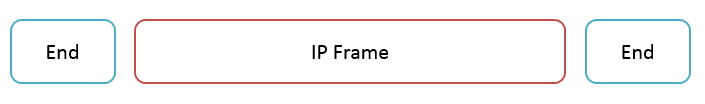
\includegraphics[width=\textwidth,height=\textheight,keepaspectratio]{ip2.png}
  \end{center}
\end{frame}

\begin{frame}{Details}
  \newpage
  \begin{center}
  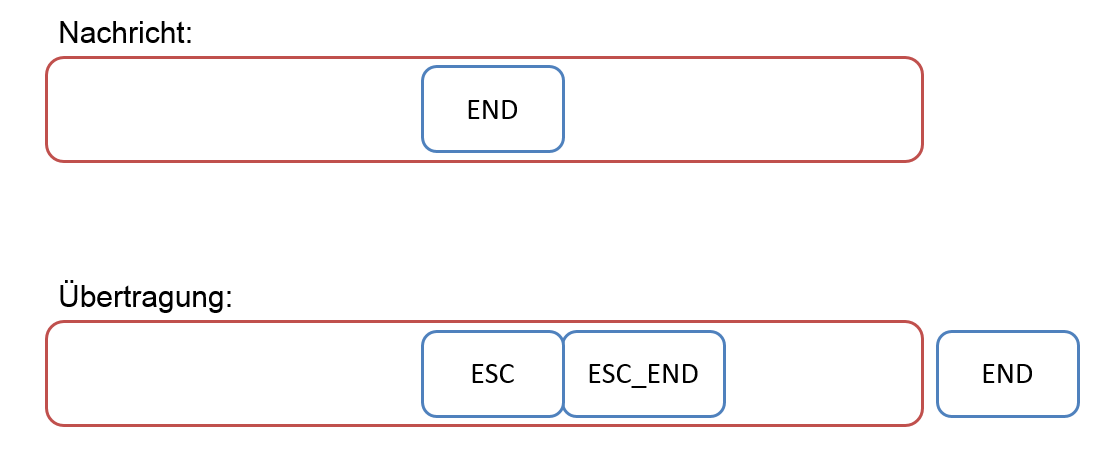
\includegraphics[width=\textwidth,height=\textheight,keepaspectratio]{escaping.png}
  \end{center}
\end{frame}

\begin{frame}{Details}
  \newpage
  \begin{center}
  \begin{itemize}
    \item END      \tabto{3cm} 0xC0 (192)
    \item ESC      \tabto{3cm} 0xDB (219)
    \item ESC\_END \tabto{3cm} 0xDC (220)
    \item ESC\_ESC \tabto{3cm} 0xDD (221)
  \end{itemize}
  \end{center}
\end{frame}

\begin{frame}{Implementierung}
  \newpage
  \begin{center}
    \lstinputlisting{src/send.c}
  \end{center}
\end{frame}

\begin{frame}{}
    \begin{block}{Vorteile}
      \begin{itemize}
        \item Sehr einfache Implementierung
        \item Sehr wenig Overhead
      \end{itemize}
    \end{block}
    \pause
    \begin{alertblock}{Nachteile}
      \begin{itemize}
        \item Steuersignale können Verbindung unterbrechen (z.B. Strg-Q, Strg-S)
        \item Keine Fehlererkennung
        \item Übertragungsrate (1,2 kbps - 19,2 kbps)
        \item Keine Meta-Daten übertragbar
      \end{itemize}
    \end{alertblock}

\end{frame}

\begin{frame}{Erweiterungs - Wünsche}
  %\begin{itemize}
    %\item Fehlerkorrektur
    %\item Daten-Komprimierung
    %\item Rechner-Adressierung
    %\item Multi-Protokoll Fähigkeit
  %\end{itemize}

  \begin{center} 
  \visible<1-4>{
    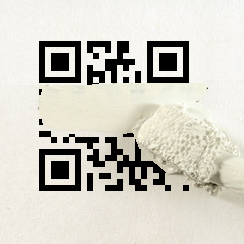
\includegraphics[width=.4\textwidth,height=.4\textheight,keepaspectratio]{erw1.png}
  }
  \quad\quad\quad
  \pause
  \visible<2-4>{
\includegraphics[width=.4\textwidth,height=.4\textheight,keepaspectratio]{erw2.png}}
  \pause
  \\
  ~\\
  \visible<3-4>{
\includegraphics[width=.4\textwidth,height=.4\textheight,keepaspectratio]{erw3.png}}
  \quad\quad\quad
  \pause
  \visible<4>{
\includegraphics[width=.4\textwidth,height=.4\textheight,keepaspectratio]{erw4.png}}
  \end{center} 
\end{frame}

\begin{frame}{Ausblick}
  \begin{block}{CSLIP (1990) \hfill RFC 1144}
    Ermöglicht Komprimierung\\
    \tabto{.9cm} Sendet nur Änderungen der TCP/IP Header. \\
    \tabto{.9cm} 40 Byte - 7 Byte pro Header im Durchschnitt
  \end{block}
  \pause
  \begin{block}{PPP (1994) \hfill RFC 1661}
    Ermöglicht:
    \begin{itemize}
      \item Ersetzung von Steuersignalen
      \item Fehlererkennung
      \item Übertragung von Netzwerk-Parametern
    \end{itemize}
  \end{block}
\end{frame}

\begin{frame}{Fragen?}
\begin{center}

\includegraphics[width=\textwidth,height=\textheight,keepaspectratio]{Fragen.jpg}
\end{center}

\end{frame}

\end{document}
